\documentclass{beamer}
\usepackage{graphicx}
\usepackage{xcolor}
\usepackage{tikz}
\usepackage{amsmath}
\usepackage{pgfplots}
\pgfplotsset{compat=1.18}

\definecolor{purpleblue}{RGB}{80, 80, 180}
\definecolor{novelPurple}{RGB}{98, 54, 255}
\definecolor{softPurple}{RGB}{180, 170, 255}
\definecolor{softGray}{RGB}{235, 235, 245}
\definecolor{lightText}{RGB}{90, 90, 110}

\usetheme{Madrid}
\usecolortheme{dolphin}
\graphicspath{{static/course_materials/}{static/hard/}{static/unit3/}{static/unit1/}{static/unit2/}{static/unit4/}{./}}

\setbeamerfont{title}{size=\Large,series=\bfseries}
\setbeamerfont{frametitle}{size=\LARGE,series=\bfseries}
\setbeamercolor{frametitle}{fg=white, bg=novelPurple}
\setbeamercolor{title}{fg=white, bg=purpleblue}

\title[Test IX]{\textbf{Test IX · Module I + II}}
\author{\textbf{Jack Zeng}}
\institute{\textcolor{white}{\textbf{Novel Prep}}}
\date{\today}

\begin{document}

\begin{frame}
    \titlepage
    \vfill
    \begin{flushright}
        \textcolor{purpleblue}{\Huge \textbf{Novel Prep}}
    \end{flushright}
\end{frame}

\begin{frame}
    \begin{tikzpicture}[remember picture, overlay]
        \shade[top color=softPurple, bottom color=softGray]
            (current page.north west) rectangle (current page.south east);
        \node[align=center] at (current page.center) {
            {\Huge\bfseries\textcolor{purpleblue}{Novel Prep}} \\[0.5cm]
            {\Large\itshape\textcolor{lightText}{Phase 3 · Mock Exam Training}}
        };
    \end{tikzpicture}
\end{frame}

\begin{frame}{Overview}
    \tableofcontents
\end{frame}

\begin{frame}
\section{Test IX}
    \begin{tikzpicture}[remember picture, overlay]
        \shade[top color=softPurple, bottom color=softGray]
            (current page.north west) rectangle (current page.south east);
        \node[align=center] at (current page.center) {
            {\LARGE\bfseries\textcolor{purpleblue}{Test IX}} \\[0.5cm]
            {\Large\itshape\textcolor{lightText}{44 questions · Module I + Module II}}
        };
    \end{tikzpicture}
\end{frame}

\begin{frame}
\section{Module I}
    \begin{tikzpicture}[remember picture, overlay]
        \shade[top color=softPurple, bottom color=softGray]
            (current page.north west) rectangle (current page.south east);
        \node[align=center] at (current page.center) {
            {\LARGE\bfseries\textcolor{purpleblue}{Module I}} \\[0.5cm]
            {\Large\itshape\textcolor{lightText}{22 Specialized Training questions}}
        };
    \end{tikzpicture}
\end{frame}

% --- Module I Question 1 ---
\begin{frame}{Question 1}
\small
One gallon of paint will cover 220 square feet of a surface. A room has a total wall area of \( w \) square feet. Which equation represents the total amount of paint \( P \), in gallons, needed to paint the walls of the room twice?
\vspace{0.35cm}
\begin{enumerate}
    \item[A.] \(\displaystyle P = \frac{w}{110}\)
    \item[B.] \(\displaystyle P = 440w\)
    \item[C.] \(\displaystyle P = \frac{w}{220}\)
    \item[D.] \(\displaystyle P = 220w\)
\end{enumerate}

\end{frame}
\begin{frame}{Answer 1}
\small
\textbf{Correct Answer:} A
\end{frame}

% --- Module I Question 2 ---
\begin{frame}{Question 2}
\small
The function \(\displaystyle f(x) = 5,470(0.64)^{\frac{x}{12}}\) gives the value, in dollars, of a certain piece of equipment after \(\displaystyle x\) months of use. If the value decreases each year by \(\displaystyle p\%\), what is the value of \(\displaystyle p\)?
\vspace{0.35cm}
\begin{enumerate}
    \item[A.] \(\displaystyle 4\)
    \item[B.] \(\displaystyle 5\)
    \item[C.] \(\displaystyle 36\)
    \item[D.] \(\displaystyle 64\)
\end{enumerate}

\end{frame}
\begin{frame}{Answer 2}
\small
\textbf{Correct Answer:} C
\end{frame}

% --- Module I Question 3 ---
\begin{frame}{Question 3}
\small
For the linear function \( f \), the table shows three values of \( x \) and their corresponding values of \( f(x) \). Function \( f \) is defined by \( f(x) = ax + b \), where \( a \) and \( b \) are constants. What is the value of \( a - b \)?

\begin{center}
\begin{tabular}{|c|c|}
\hline
\(\displaystyle x\) \& \(\displaystyle f(x)\) \\
\hline
1 \& -64 \\
\hline
2 \& 0 \\
\hline
3 \& 64 \\
\hline
\end{tabular}
\end{center}
\vspace{0.35cm}
\begin{enumerate}
    \item[A.] \(\displaystyle -64\)
    \item[B.] \(\displaystyle 62\)
    \item[C.] \(\displaystyle 128\)
    \item[D.] \(\displaystyle 192\)
\end{enumerate}

\end{frame}
\begin{frame}{Answer 3}
\small
\textbf{Correct Answer:} D
\end{frame}

% --- Module I Question 4 ---
\begin{frame}{Question 4}
\small
Let the function \(\displaystyle p\) be defined as \(\displaystyle p(x) = \dfrac{(x - c)^2 + 160}{2c}\), where \(\displaystyle c\) is a constant. If \(\displaystyle p(c) = 10\), what is the value of \(\displaystyle p(12)\)?
\vspace{0.35cm}
\begin{enumerate}
    \item[A.] \(\displaystyle 10.00\)
    \item[B.] \(\displaystyle 10.25\)
    \item[C.] \(\displaystyle 10.75\)
    \item[D.] \(\displaystyle 11.00\)
\end{enumerate}

\end{frame}
\begin{frame}{Answer 4}
\small
\textbf{Correct Answer:} D
\end{frame}

% --- Module I Question 5 ---
\begin{frame}{Question 5}
\small
Jennifer bought a box of Crunchy Grain cereal. The nutrition facts on the box state that a serving size of the cereal is \(\displaystyle \frac{3}{4}\) cup and provides 210 calories, 50 of which are calories from fat. In addition, each serving of the cereal provides 180 milligrams of potassium, which is 5\% of the daily allowance for adults. If \(\displaystyle p\) percent of an adult’s daily allowance of potassium is provided by \(\displaystyle x\) servings of Crunchy Grain cereal per day, which of the following expresses \(\displaystyle p\) in terms of \(\displaystyle x\)?
\vspace{0.35cm}
\begin{enumerate}
    \item[A.] \(\displaystyle p = 0.5x\)
    \item[B.] \(\displaystyle p = 5x\)
    \item[C.] \(\displaystyle p = (0.05)^x\)
    \item[D.] \(\displaystyle p = (1.05)^x\)
\end{enumerate}

\end{frame}
\begin{frame}{Answer 5}
\small
\textbf{Correct Answer:} B
\end{frame}

% --- Module I Question 6 ---
\begin{frame}{Question 6}
\small
According to data provided by the US Department of Energy, the average price per gallon of regular gasoline in the United States from September 1, 2014, to December 1, 2014, is modeled by the function \( F \) defined below, where \( F(x) \) is the average price per gallon \( x \) months after September 1.

\[
F(x) = 2.74 - 0.19(x - 3)
\]

The constant 2.74 in this function estimates which of the following?
\vspace{0.35cm}
\begin{enumerate}
    \item[A.] The average monthly decrease in the price per gallon
    \item[B.] The difference in the average price per gallon from September 1, 2014, to December 1, 2014
    \item[C.] The average price per gallon on September 1, 2014
    \item[D.] The average price per gallon on December 1, 2014
\end{enumerate}

\end{frame}
\begin{frame}{Answer 6}
\small
\textbf{Correct Answer:} D
\end{frame}

% --- Module I Question 7 ---
\begin{frame}{Question 7}
\small
What is the minimum value of the function \(\displaystyle f\) defined by \(\displaystyle f(x) = (x - 2)^2 - 4\)?
\vspace{0.35cm}
\begin{enumerate}
    \item[A.] \(\displaystyle -4\)
    \item[B.] \(\displaystyle -2\)
    \item[C.] \(\displaystyle 2\)
    \item[D.] \(\displaystyle 4\)
\end{enumerate}

\end{frame}
\begin{frame}{Answer 7}
\small
\textbf{Correct Answer:} A
\end{frame}

% --- Module I Question 8 ---
\begin{frame}{Question 8}
\small
The equation \(\displaystyle x^2 + (y - 2)^2 = 36\) represents circle \(\displaystyle A\). Circle \(\displaystyle B\) is obtained by shifting circle \(\displaystyle A\) down \(\displaystyle 4\) units in the \(\displaystyle xy\)-plane. Which of the following equations represents circle \(\displaystyle B\)?
\vspace{0.35cm}
\begin{enumerate}
    \item[A.] \(\displaystyle x^2 + (y - 6)^2 = 36\)
    \item[B.] \(\displaystyle x^2 + (y + 2)^2 = 36\)
    \item[C.] \(\displaystyle (x - 4)^2 + (y - 2)^2 = 36\)
    \item[D.] \(\displaystyle (x + 4)^2 + (y - 2)^2 = 36\)
\end{enumerate}

\end{frame}
\begin{frame}{Answer 8}
\small
\textbf{Correct Answer:} A
\end{frame}

% --- Module I Question 9 ---
\begin{frame}{Question 9}
\small
If \( \frac{x + 6}{3} = \frac{x + 6}{13} \), the value of \( x + 6 \) is between which of the following pairs of values?
\vspace{0.35cm}
\begin{enumerate}
    \item[A.] \(-7\) and \(-3\)
    \item[B.] \(-2\) and 2
    \item[C.] 2 and 7
    \item[D.] 8 and 13
\end{enumerate}

\end{frame}
\begin{frame}{Answer 9}
\small
\textbf{Correct Answer:} B
\end{frame}

% --- Module I Question 10 ---
\begin{frame}{Question 10}
\small
Kao measured the temperature of a cup of hot chocolate placed in a room with a constant temperature of 70 degrees Fahrenheit (°F). The temperature of the hot chocolate was \(\displaystyle 185^\circ\)F at 6:00 p.m. when it started cooling. The temperature of the hot chocolate was \(\displaystyle 156^\circ\)F at 6:05 p.m. and \(\displaystyle 135^\circ\)F at 6:10 p.m. The hot chocolate’s temperature continued to decrease. Of the following functions, which best models the temperature \(\displaystyle T(m)\), in degrees Fahrenheit, of Kao’s hot chocolate \(\displaystyle m\) minutes after it started cooling?
\vspace{0.35cm}
\begin{enumerate}
    \item[A.] \(\displaystyle T(m) = 185(1.25)^m\)
    \item[B.] \(\displaystyle T(m) = 185(0.85)^m\)
    \item[C.] \(\displaystyle T(m) = (185 - 70)(0.75)^{\frac{m}{5}}\)
    \item[D.] \(\displaystyle T(m) = 70 + 115(0.75)^{\frac{m}{5}}\)
\end{enumerate}

\end{frame}
\begin{frame}{Answer 10}
\small
\textbf{Correct Answer:} D
\end{frame}

% --- Module I Question 11 ---
\begin{frame}{Question 11}
\small
A shipping service restricts the dimensions of the boxes it will ship for a certain type of service. The restriction states that for boxes shaped like rectangular prisms, the sum of the perimeter of the base of the box and the height of the box cannot exceed 130 inches. The perimeter of the base is determined using the width and length of the box. If a box has a height of 60 inches and its length is 2.5 times the width, which inequality shows the allowable width \( x \), in inches, of the box?
\vspace{0.35cm}
\begin{enumerate}
    \item[A.] \(\displaystyle 0 \lt x \leq 10\)
    \item[B.] \(\displaystyle 0 \lt x \leq 11\frac{2}{3}\)
    \item[C.] \(\displaystyle 0 \lt x \leq 17\frac{1}{2}\)
    \item[D.] \(\displaystyle 0 \lt x \leq 20\)
\end{enumerate}

\end{frame}
\begin{frame}{Answer 11}
\small
\textbf{Correct Answer:} A
\end{frame}

% --- Module I Question 12 ---
\begin{frame}{Question 12}
\small
\[f(x) = 9(4)^x\]

The function \(\displaystyle f\) is defined by the given equation. If \(\displaystyle g(x) = f(x + 2)\), which of the following equations defines the function \(\displaystyle g\)?
\vspace{0.35cm}
\begin{enumerate}
    \item[A.] \(\displaystyle g(x) = 18(4)^x\)
    \item[B.] \(\displaystyle g(x) = 144(4)^x\)
    \item[C.] \(\displaystyle g(x) = 18(8)^x\)
    \item[D.] \(\displaystyle g(x) = 81(16)^x\)
\end{enumerate}

\end{frame}
\begin{frame}{Answer 12}
\small
\textbf{Correct Answer:} B
\end{frame}

% --- Module I Question 13 ---
\begin{frame}{Question 13}
\small
A data set of 27 different numbers has a mean of 33 and a median of 33. A new data set is created by adding 7 to each number in the original data set that is greater than the median and subtracting 7 from each number in the original data set that is less than the median. Which of the following measures does NOT have the same value in both the original and new data sets?
\vspace{0.35cm}
\begin{enumerate}
    \item[A.] Median
    \item[B.] Mean
    \item[C.] Sum of the numbers
    \item[D.] Standard deviation
\end{enumerate}

\end{frame}
\begin{frame}{Answer 13}
\small
\textbf{Correct Answer:} D
\end{frame}

% --- Module I Question 14 ---
\begin{frame}{Question 14}
\small
An economist modeled the demand \( Q \) for a certain product as a linear function of the selling price \( P \). The demand was 20,000 units when the selling price was \(\$40\) per unit, and the demand was 15,000 units when the selling price was \(\$60\) per unit. Based on the model, what is the demand, in units, when the selling price is \(\$55\) per unit?
\vspace{0.35cm}
\begin{enumerate}
    \item[A.] 16,250
    \item[B.] 16,500
    \item[C.] 16,750
    \item[D.] 17,500
\end{enumerate}

\end{frame}
\begin{frame}{Answer 14}
\small
\textbf{Correct Answer:} A
\end{frame}

% --- Module I Question 15 ---
\begin{frame}{Question 15}
\small
Function \(\displaystyle f\) is defined by \(\displaystyle f(x) = (x + 6)(x + 5)(x + 1)\). Function \(\displaystyle g\) is defined by \(\displaystyle g(x) = f(x - 1)\). The graph of \(\displaystyle y = g(x)\) in the \(\displaystyle xy\)-plane has \(\displaystyle x\)-intercepts at \(\displaystyle (a, 0)\), \(\displaystyle (b, 0)\), and \(\displaystyle (c, 0)\), where \(\displaystyle a\), \(\displaystyle b\), and \(\displaystyle c\) are distinct constants. What is the value of \(\displaystyle a + b + c\)?
\vspace{0.35cm}
\begin{enumerate}
    \item[A.] \(\displaystyle -15\)
    \item[B.] \(\displaystyle -9\)
    \item[C.] \(\displaystyle 11\)
    \item[D.] \(\displaystyle 15\)
\end{enumerate}

\end{frame}
\begin{frame}{Answer 15}
\small
\textbf{Correct Answer:} B
\end{frame}

% --- Module I Question 16 ---
\begin{frame}{Question 16}
\small
A circle in the \(\displaystyle xy\)-plane has its center at \(\displaystyle (-4, -6)\). Line \(\displaystyle k\) is tangent to this circle at the point \(\displaystyle (-7, -7)\). What is the slope of line \(\displaystyle k\)?
\vspace{0.35cm}
\begin{enumerate}
    \item[A.] \(\displaystyle -3\)
    \item[B.] \(\displaystyle -\dfrac{1}{3}\)
    \item[C.] \(\displaystyle \dfrac{1}{3}\)
    \item[D.] \(\displaystyle 3\)
\end{enumerate}

\end{frame}
\begin{frame}{Answer 16}
\small
\textbf{Correct Answer:} A
\end{frame}

% --- Module I Question 17 ---
\begin{frame}{Question 17}
\small
A window repair specialist charges \textbf{\(\$220\)} for the first two hours of repair plus an hourly fee for each additional hour. The total cost for 5 hours of repair is \textbf{\(\$400\)}. Which function \( f \) gives the total cost, in dollars, for \( x \) hours of repair, where \( x \geq 2 \)?
\vspace{0.35cm}
\begin{enumerate}
    \item[A.] \(\displaystyle f(x) = 60x + 100\)
    \item[B.] \(\displaystyle f(x) = 60x + 220\)
    \item[C.] \(\displaystyle f(x) = 80x\)
    \item[D.] \(\displaystyle f(x) = 80x + 220\)
\end{enumerate}

\end{frame}
\begin{frame}{Answer 17}
\small
\textbf{Correct Answer:} A
\end{frame}

% --- Module I Question 18 ---
\begin{frame}{Question 18}
\small
The functions f and g are defined by the given equation, where \(\displaystyle  x \geq0\). Which function shows a maximum value as a constant or coefficient for \(\displaystyle x \geq 0\)?

\begin{enumerate}
    \item[I.] \(\displaystyle f(x) = 33(0.4)^{x + 3}\)
    \item[II.] \(\displaystyle g(x) = 33(0.16)(0.4)^{x - 2}\).
\end{enumerate}
\vspace{0.35cm}
\begin{enumerate}
    \item[A.] I only
    \item[B.] II only
    \item[C.] I and II
    \item[D.] Neither I nor II
\end{enumerate}

\end{frame}
\begin{frame}{Answer 18}
\small
\textbf{Correct Answer:} B
\end{frame}

% --- Module I Question 19 ---
\begin{frame}{Question 19}
\small
For the function \( f \), if \( f(3x) = x - 6 \) for all values of \( x \), what is the value of \( f(6) \)?
\vspace{0.35cm}
\begin{enumerate}
    \item[A.] \(\displaystyle -6\)
    \item[B.] \(\displaystyle -4\)
    \item[C.] \(\displaystyle 0\)
    \item[D.] \(\displaystyle 2\)
\end{enumerate}

\end{frame}
\begin{frame}{Answer 19}
\small
\textbf{Correct Answer:} B
\end{frame}

% --- Module I Question 20 ---
\begin{frame}{Question 20}
\small
\(\displaystyle P(t) = 290(1.04)^{\frac{4}{6}t}\) models the population, in thousands, of a certain city \(\displaystyle t\) years after 2005. The population increases by \(\displaystyle n\%\) every 18 months. What is the value of \(\displaystyle n\)?
\vspace{0.35cm}
\begin{enumerate}
    \item[A.] \(\displaystyle 0.38\)
    \item[B.] \(\displaystyle 1.04\)
    \item[C.] \(\displaystyle 4\)
    \item[D.] \(\displaystyle 6\)
\end{enumerate}

\end{frame}
\begin{frame}{Answer 20}
\small
\textbf{Correct Answer:} C
\end{frame}

% --- Module I Question 21 ---
\begin{frame}{Question 21}
\small
\begin{center}
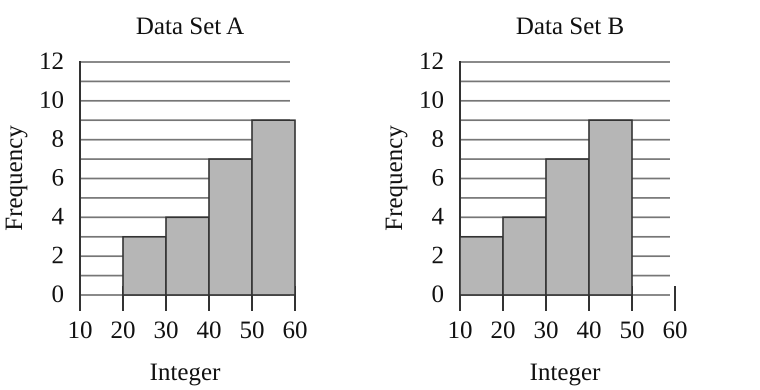
\includegraphics[width=0.82\linewidth]{static/unit3/unit3_histograms_ab.svg}
\end{center}

Two data sets of 23 integers each are summarized in the histograms shown. For each of the histograms, the first interval represents the frequency of integers greater than or equal to 10, but less than 20. The second interval represents the frequency of integers greater than or equal to 20, but less than 30, and so on. What is the smallest possible difference between the mean of data set A and the mean of data set B?
\vspace{0.35cm}
\begin{enumerate}
    \item[A.] 0
    \item[B.] 1
    \item[C.] 10
    \item[D.] 23
\end{enumerate}

\end{frame}
\begin{frame}{Answer 21}
\small
\textbf{Correct Answer:} B
\end{frame}

% --- Module I Question 22 ---
\begin{frame}{Question 22}
\small
A cube has an edge length of 68 inches. A solid sphere with a radius of 34 inches is inside the cube, such that the sphere touches the center of each face of the cube. To the nearest cubic inch, what is the volume of the space in the cube not taken up by the sphere?
\vspace{0.35cm}
\begin{enumerate}
    \item[A.] 149,796
    \item[B.] 164,500
    \item[C.] 190,955
    \item[D.] 310,800
\end{enumerate}

\end{frame}
\begin{frame}{Answer 22}
\small
\textbf{Correct Answer:} A
\end{frame}

\begin{frame}
\section{Module II}
    \begin{tikzpicture}[remember picture, overlay]
        \shade[top color=softPurple, bottom color=softGray]
            (current page.north west) rectangle (current page.south east);
        \node[align=center] at (current page.center) {
            {\LARGE\bfseries\textcolor{purpleblue}{Module II}} \\[0.5cm]
            {\Large\itshape\textcolor{lightText}{22 Hard Problem Drill questions}}
        };
    \end{tikzpicture}
\end{frame}

% --- Module II Question 1 ---
\begin{frame}{Question 1}
\small
In the given equation, \(c\) is a constant. The equation has infinitely many solutions. What is the value of \(c\)?
\[
18(x+5)=2(x+c)+16x
\]
\vspace{0.35cm}
\begin{enumerate}
    \item[A.] 90
    \item[B.] 45
    \item[C.] 10
    \item[D.] 5
\end{enumerate}
\end{frame}
\begin{frame}{Answer 1}
\small
\textbf{Correct Answer:} B
\end{frame}

% --- Module II Question 2 ---
\begin{frame}{Question 2}
\small
Hannah and Wyatt are saving money to purchase a car. Hannah saves \(\frac{1}{5}\) of her salary each month, and Wyatt saves \(\frac{2}{7}\) of his salary each month. Together, they save a total of \$3{,}270 from their monthly salaries each month. If \(h\) and \(w\) represent Hannah's and Wyatt's monthly salaries, in dollars, respectively, which equation shows the relationship between \(h\) and \(w\)?
\vspace{0.35cm}
\begin{enumerate}
    \item[A.] $h+w=3{,}270$
    \item[B.] $h+2w=3{,}270$
    \item[C.] $10h+7w=114{,}450$
    \item[D.] $7h+10w=114{,}450$
\end{enumerate}
\end{frame}
\begin{frame}{Answer 2}
\small
\textbf{Correct Answer:} D
\end{frame}

% --- Module II Question 3 ---
\begin{frame}{Question 3}
\small
The figure shows a rectangular pool surrounded by a concrete path that is \(x\) feet (ft) wide on all sides. The pool is \(21\) ft long and \(11\) ft wide. The area of the concrete path is \(144\,\text{ft}^2\). What is the value of \(x\)?

\begin{center}
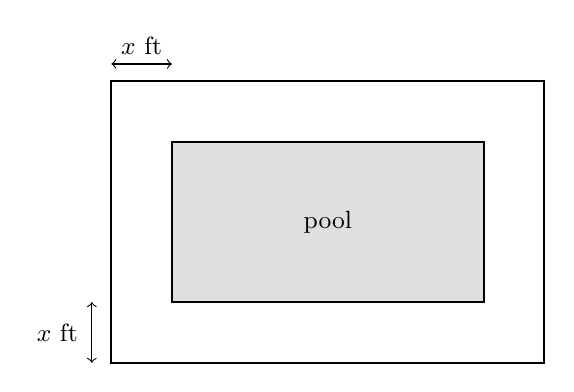
\begin{tikzpicture}[scale=0.55]
  \draw[thick] (0,0) rectangle (10,6.5);
  \fill[gray!25] (1.4,1.4) rectangle (8.6,5.1);
  \draw[thick] (1.4,1.4) rectangle (8.6,5.1);
  \node at (5,3.25) {\small pool};
  \draw[<->] (-0.45,1.4) -- (-0.45,0);
  \node[left] at (-0.55,0.7) {\small \(x\) ft};
  \draw[<->] (1.4,6.9) -- (0,6.9);
  \node[above] at (0.7,6.9) {\small \(x\) ft};
\end{tikzpicture}\\[0.2em]
\textit{Note: Figure not drawn to scale.}
\end{center}
\vspace{0.35cm}
\begin{enumerate}
    \item[A.] 2
    \item[B.] 4
    \item[C.] 18
    \item[D.] 36
\end{enumerate}
\end{frame}
\begin{frame}{Answer 3}
\small
\textbf{Correct Answer:} A
\end{frame}

% --- Module II Question 4 ---
\begin{frame}{Question 4}
\small
A wildlife biologist counted bald eagles at a nature preserve every day for 21 days. The results are shown in the table below as data set A.

\begin{center}
\begin{tabular}{|c|c|}
\hline
\textbf{Number of bald eagles} & \textbf{Number of days}\\
\hline
0 & 1\\
1 & 3\\
2 & 4\\
3 & 5\\
4 & 4\\
5 & 3\\
19 & 1\\
\hline
\end{tabular}
\end{center}

The value 19 was recorded in error and is removed from data set A to create data set B. Which of the following best compares the median of data set A and the median of data set B?
\vspace{0.35cm}
\begin{enumerate}
    \item[A.] The median of data set B is less than the median of data set A.
    \item[B.] The median of data set B is equal to the median of data set A.
    \item[C.] The median of data set B is greater than the median of data set A.
    \item[D.] There is not enough information to compare the medians of the two data sets.
\end{enumerate}
\end{frame}
\begin{frame}{Answer 4}
\small
\textbf{Correct Answer:} B
\end{frame}

% --- Module II Question 5 ---
\begin{frame}{Question 5}
\small
The equation \(3x - 9 = 12\) is true for which value of \(x\)?
\vspace{0.35cm}
\begin{enumerate}
    \item[A.] $1$
    \item[B.] $5$
    \item[C.] $7$
    \item[D.] $21$
\end{enumerate}
\end{frame}
\begin{frame}{Answer 5}
\small
\textbf{Correct Answer:} C
\end{frame}

% --- Module II Question 6 ---
\begin{frame}{Question 6}
\small
\[
f(x)=4^{-5(x+1)}
\]
Which of the following equivalent forms of the given function \(f\) displays, as the base or the coefficient, the \(y\)-coordinate of the \(y\)-intercept of the graph of \(y=f(x)\) in the \(xy\)-plane?
\vspace{0.35cm}
\begin{enumerate}
    \item[A.] $f(x)=\dfrac{1}{1{,}024}\left(\dfrac{1}{4}\right)^{5x}$
    \item[B.] $f(x)=\left(\dfrac{1}{4}\right)^{5x+5}$
    \item[C.] $f(x)=4^{-5x-5}$
    \item[D.] $f(x)=1{,}024^{-x-1}$
\end{enumerate}
\end{frame}
\begin{frame}{Answer 6}
\small
\textbf{Correct Answer:} A
\end{frame}

% --- Module II Question 7 ---
\begin{frame}{Question 7}
\small
One of the equations in a system of two linear equations is given:  
\[
31(x - n) = 31y + 31n
\]  
where \(n\) is a positive constant.  
The system has no solution. Which equation could be the second equation in this system?
\vspace{0.35cm}
\begin{enumerate}
    \item[A.] $3x - 3y = 6n$
    \item[B.] $3x + 3y = 3n$
    \item[C.] $3x + 3y = 6n$
    \item[D.] $3x - 3y = 3n$
\end{enumerate}
\end{frame}
\begin{frame}{Answer 7}
\small
\textbf{Correct Answer:} D
\end{frame}

% --- Module II Question 8 ---
\begin{frame}{Question 8}
\small
The given equation is one equation in a system of two linear equations.  
If the system of equations has at least one solution, which of the following equations could be the other equation in the system?

\[
7x + 5y = 2
\]

\begin{itemize}
    \item[I.] \(10.5x + 7.5y = 3\)
    \item[II.] \(10.5x - 7.5y = 3\)
\end{itemize}
\vspace{0.35cm}
\begin{enumerate}
    \item[A.] I only
    \item[B.] II only
    \item[C.] I and II
    \item[D.] Neither I nor II
\end{enumerate}
\end{frame}
\begin{frame}{Answer 8}
\small
\textbf{Correct Answer:} C
\end{frame}

% --- Module II Question 9 ---
\begin{frame}{Question 9}
\small
For each real number \( r \), which of the following points lies on the graph of each equation in the \( xy \)-plane for the given system?
\[
\begin{aligned}
2x + 3y &= 7 \\
10x + 15y &= 35
\end{aligned}
\]
\vspace{0.35cm}
\begin{enumerate}
    \item[A.] $\left(\frac{7}{5} + r, -\frac{7}{5} + 35 \right)$
    \item[B.] $\left(-\frac{3r}{2} + \frac{7}{2}, r \right)$
    \item[C.] $\left(r, \frac{2r}{3} + \frac{7}{3} \right)$
    \item[D.] $\left(r, -\frac{3r}{2} + \frac{7}{2} \right)$
\end{enumerate}
\end{frame}
\begin{frame}{Answer 9}
\small
\textbf{Correct Answer:} B
\end{frame}

% --- Module II Question 10 ---
\begin{frame}{Question 10}
\small
In the \(xy\)-plane, the graph of the linear function \(f\) has a negative slope
and a \(y\)-intercept at \((0,k)\), where \(k\) is a positive constant. Which of
the following must be true?
\[
\begin{array}{ll}
\text{I.} & \text{If }a>b,\text{ then }f(a)<f(b).\\
\text{II.} & \text{If }a<0,\text{ then }f(a)>k.\\
\text{III.} & \text{If }a>0,\text{ then }f(a)>0.
\end{array}
\]
\vspace{0.35cm}
\begin{enumerate}
    \item[A.] I and II only
    \item[B.] I and III only
    \item[C.] II and III only
    \item[D.] I, II, and III
\end{enumerate}
\end{frame}
\begin{frame}{Answer 10}
\small
\textbf{Correct Answer:} A
\end{frame}

% --- Module II Question 11 ---
\begin{frame}{Question 11}
\small
In the \(xy\)-plane, what is the slope of the line that passes through the points \((1,2)\) and \((5,10)\)?
\vspace{0.35cm}
\begin{enumerate}
    \item[A.] $1$
    \item[B.] $2$
    \item[C.] $4$
    \item[D.] $8$
\end{enumerate}
\end{frame}
\begin{frame}{Answer 11}
\small
\textbf{Correct Answer:} B
\end{frame}

% --- Module II Question 12 ---
\begin{frame}{Question 12}
\small
The function $f$ is defined by the given equation: 
\[
f(x) = x^2 - 4x - 320
\]
Which of the following equivalent forms of the equation displays the minimum value of the function as a constant or coefficient?
\vspace{0.35cm}
\begin{enumerate}
    \item[A.] $f(x) = x^2 - 4(x + 80)$
    \item[B.] $f(x) = (x - 2)^2 + (-324)$
    \item[C.] $f(x) = x(x - 4) + (-320)$
    \item[D.] $f(x) = (x + 16)(x - 20)$
\end{enumerate}
\end{frame}
\begin{frame}{Answer 12}
\small
\textbf{Correct Answer:} B
\end{frame}

% --- Module II Question 13 ---
\begin{frame}{Question 13}
\small
At different times on a certain day, a manager at a theme park recorded the number of visitors.  
An exponential model gives the estimated number of visitors, $V$, at the theme park $t$ hours after the theme park opened, where $t \leq 3$.  
Based on the model, 80 visitors were estimated to be at the theme park when it opened,  
and every 30 minutes the estimated number of visitors increased by 150\% of the number 30 minutes earlier.  
Which of the following equations best represents this model?
\vspace{0.35cm}
\begin{enumerate}
    \item[A.] $V = 80(2.5)^{2t}$
    \item[B.] $V = 80(2.5)^{\frac{t}{30}}$
    \item[C.] $V = 80(1.5)^{2t}$
    \item[D.] $V = 80(1.5)^{\frac{t}{30}}$
\end{enumerate}
\end{frame}
\begin{frame}{Answer 13}
\small
\textbf{Correct Answer:} A
\end{frame}

% --- Module II Question 14 ---
\begin{frame}{Question 14}
\small
An economist fits a quadratic revenue model \(y = f(x)\) that breaks even at two production levels. The function \(f\) is defined by
\[
f(x) = ax^2 + bx + c,
\]
where \(a, b, c\) are constants. The graph of \(y = f(x)\) passes through the points \((9, 0)\) and \((-2, 0)\). If \(a\) is an integer greater than 1, which of the following could be the value of \(a + b\)?
\vspace{0.35cm}
\begin{enumerate}
    \item[A.] \(8\)
    \item[B.] \(7\)
    \item[C.] \(-6\)
    \item[D.] \(-12\)
\end{enumerate}
\end{frame}
\begin{frame}{Answer 14}
\small
\textbf{Correct Answer:} D
\end{frame}

% --- Module II Question 15 ---
\begin{frame}{Question 15}
\small
A savings balance is modeled by an exponential function of time. In the given function, \(b\) is a positive constant. For every increase in the value of \(x\) by 1, the value of \(f(x)\) increases by \(c\%\), where \(0 < c < 100\).

Which expression gives the value of \(c\) in terms of \(b\)?
\[
f(x) = 66(b)^x
\]
\vspace{0.35cm}
\begin{enumerate}
    \item[A.] \(1 + \dfrac{b}{100}\)
    \item[B.] \(b + 100\)
    \item[C.] \(100(b + 1)\)
    \item[D.] \(100(b - 1)\)
\end{enumerate}
\end{frame}
\begin{frame}{Answer 15}
\small
\textbf{Correct Answer:} D
\end{frame}

% --- Module II Question 16 ---
\begin{frame}{Question 16}
\small
The exponential function \(f\) is defined by
\[
f(x) = ab^x,
\]
where \(a\) and \(b\) are positive constants.
If \(f(s) = t\) and \(f(s + 1) = t - 0.87t\), where \(s\) and \(t\) are constants, what is the value of \(b\)?
\vspace{0.35cm}
\begin{enumerate}
    \item[A.] 0.13
    \item[B.] 0.87
    \item[C.] 1.13
    \item[D.] 1.87
\end{enumerate}
\end{frame}
\begin{frame}{Answer 16}
\small
\textbf{Correct Answer:} A
\end{frame}

% --- Module II Question 17 ---
\begin{frame}{Question 17}
\small
Let \(f(x) = x^3 - 9x\) and \(g(x) = x^2 - 2x - 3\). Which of the following expressions is equivalent to \(\dfrac{f(x)}{g(x)}\) for \(x > 3\)?
\vspace{0.35cm}
\begin{enumerate}
    \item[A.] $\dfrac{1}{x + 1}$
    \item[B.] $\dfrac{x + 3}{x + 1}$
    \item[C.] $\dfrac{x(x - 3)}{x + 1}$
    \item[D.] $\dfrac{x(x + 3)}{x + 1}$
\end{enumerate}
\end{frame}
\begin{frame}{Answer 17}
\small
\textbf{Correct Answer:} D
\end{frame}

% --- Module II Question 18 ---
\begin{frame}{Question 18}
\small
The function \(f(x) = 4x^2 + 64x + 262\) is defined, and \(g(x) = f(x + 5)\). For what value of \(x\) does \(g(x)\) reach its minimum?
\vspace{0.35cm}
\begin{enumerate}
    \item[A.] $-13$
    \item[B.] $-8$
    \item[C.] $-5$
    \item[D.] $-3$
\end{enumerate}
\end{frame}
\begin{frame}{Answer 18}
\small
\textbf{Correct Answer:} A
\end{frame}

% --- Module II Question 19 ---
\begin{frame}{Question 19}
\small
For data set A, the table summarizes the distribution of the number of pieces of mail received by a business each day during a period of 11 days.

\[
\begin{array}{|c|c|}
\hline
\text{Pieces of mail} & \text{Days} \\
\hline
0 & 2 \\
4 & 2 \\
5 & 2 \\
6 & 2 \\
7 & 1 \\
8 & 1 \\
17 & 1 \\
\hline
\end{array}
\]

The data value $17$ is removed from data set A to create data set B, which consists of the remaining 10 data values.  
Which statement best compares the median of data set A and the median of data set B?
\vspace{0.35cm}
\begin{enumerate}
    \item[A.] The median of data set B is less than the median of data set A.
    \item[B.] The median of data set B is greater than the median of data set A.
    \item[C.] The median of data set B is equal to the median of data set A.
    \item[D.] There is not enough information to compare the medians of the two data sets.
\end{enumerate}
\end{frame}
\begin{frame}{Answer 19}
\small
\textbf{Correct Answer:} C
\end{frame}

% --- Module II Question 20 ---
\begin{frame}{Question 20}
\small
\begin{center}
\begin{tabular}{|c|c|}
\hline
\textbf{Data} & \textbf{Frequency}\\
\hline
1 & 2\\
2 & 5\\
3 & 6\\
4 & 5\\
5 & 2\\
\hline
\end{tabular}
\end{center}

The frequency table above summarizes data set A. 
Data set B is created by multiplying all of the values in data set A by $2$. 
Which of the following must be true?

\begin{itemize}
\item[I.] The difference between the mean and median of data set B is $0$.
\item[II.] The standard deviation of data set B is equal to the standard deviation of data set A.
\item[III.] The range of data set B is double the range of data set A.
\end{itemize}
\vspace{0.35cm}
\begin{enumerate}
    \item[A.] I and II only
    \item[B.] II and III only
    \item[C.] I and III only
    \item[D.] I, II, and III
\end{enumerate}
\end{frame}
\begin{frame}{Answer 20}
\small
\textbf{Correct Answer:} C
\end{frame}

% --- Module II Question 21 ---
\begin{frame}{Question 21}
\small
In isosceles triangle $ABC$, sides $AB$ and $AC$ are congruent. Point $D$ divides side $BC$ such that the length of $\overline{BD}$ is $\dfrac{4}{7}$ of the length of $\overline{BC}$. Point $E$ lies on side $AB$ and point $F$ lies on side $AC$ such that when segments $\overline{DE}$ and $\overline{DF}$ are drawn, angle $\angle BED$ is congruent to angle $\angle CFD$. If the length of $\overline{BE}$ is $8$, what is the length of $\overline{CF}$?
\vspace{0.35cm}
\begin{enumerate}
    \item[A.] 6
    \item[B.] 14
    \item[C.] 32
    \item[D.] 56
\end{enumerate}
\end{frame}
\begin{frame}{Answer 21}
\small
\textbf{Correct Answer:} A
\end{frame}

% --- Module II Question 22 ---
\begin{frame}{Question 22}
\small
Triangle $ABC$ is similar to triangle $DEF$, where $A$ corresponds to $D$ and $C$ corresponds to $F$.  
Angles $C$ and $F$ are right angles.  
If $\tan(A) = \sqrt{5}$ and $DF = 53$, what is the length of $DE$?
\vspace{0.35cm}
\begin{enumerate}
    \item[A.] $\dfrac{53\sqrt{3}}{5}$
    \item[B.] $\dfrac{53\sqrt{3}}{2}$
    \item[C.] $53\sqrt{6}$
    \item[D.] $106$
\end{enumerate}
\end{frame}
\begin{frame}{Answer 22}
\small
\textbf{Correct Answer:} C
\end{frame}

\begin{frame}{}
    \begin{tikzpicture}[remember picture, overlay]
        \shade[top color=novelPurple!40, bottom color=white]
            (current page.north west) rectangle (current page.south east);
        \fill[white, opacity=0.15] (current page.center) circle (5cm);
        \foreach \x in {1,2,3,4,5} {
            \fill[novelPurple, opacity=0.12] (rand*10-5, rand*7-3.5) circle (0.1+\x*0.05);
        }
    \end{tikzpicture}
    \centering
    \vspace{5em}
    {\Huge \textbf{\textcolor{novelPurple}{Thank You!}}} \\[1em]
    {\large \textcolor{gray}{We appreciate your time and focus.}} \\[3em]
    {\LARGE \textbf{\textcolor{novelPurple}{\textsf{Novel Prep}}}}
    \vfill
\end{frame}

\end{document}
